\documentclass[10pt,a4paper,oneside]{article}
\usepackage[utf8]{inputenc}
\usepackage{draftwatermark} % 设置水印
\SetWatermarkText{DNV Group} % 水印内容
\usepackage{amsmath}
\usepackage{amsfonts}
\usepackage{amssymb}
\usepackage{graphicx}
\usepackage{breqn}
\usepackage{tikz} % system block diagram
\usepackage{textcomp}
\usetikzlibrary{shapes,arrows} % system block diagram
\usepackage{booktabs}
\usepackage[framed,numbered,autolinebreaks,useliterate]{mcode} % matlab code block
\author{Yangang Cao}
\date{February 19, 2019}
\newcommand{\degree}{^\circ}
\tikzset{
	delay/.style    = {draw, thick, rectangle, minimum height = 3em,
		minimum width = 3em},
	sum/.style      = {draw, circle, node distance = 2cm}, 
	prod/.style     = {draw, circle, node distance = 2cm},
	input/.style    = {coordinate}, % Input
	output/.style  = {coordinate} % Output
}
% Defining string as labels of certain blocks.
\newcommand{\product}{$\displaystyle \times$}
\newcommand{\delay}{\large$z^{-1}$}
\begin{document}

\title{Second-Order Peak Filter Design}
\maketitle 
In contrast to low/highpass and bandpass/reject filters, which attenuate the audio spectrum above or below a cut-off frequency, equalizers shape the audio spectrum by enhancing certain frequency bands while others remain unaffected. They are typically built by a series connection of first-and second-order shelving and peak filters, which are controlled independently.

Peak filters boost or cut mid-frequency bands with parameters center frequency $fc$,
bandwidth $fb$ and gain $G$. One often-used filter type is the constant Q peak filter. The Q factor is defined by the ratio of the bandwidth to center frequency $Q = \frac{fc}{fb}$. The center frequency of peak filters is then tuned while keeping the Q factor constant. This means that the bandwidth is increased when the center frequency is increased and vice versa.

Similarly to first-order shelving filters, a second-order peak filter based on second-order allpass filter is given by the transfer function
\[
H(z) = 1 + \frac{H_0}{2}[1 - A_2(z)],
\]
where
\[
A_2(z) = \frac{-c_{B/C} + d(1 - c_{B/C})z^{-1} + z^{-2}}{1 + d(1 - c_{B/C})z^{-1} - c_{B/C}z^{-2}}
\]
is a second-order allpass filter. The block diagram in following figure shows the second-order peak filter, the part of $A_2(z)$ can be reviewed in previous document,
\begin{center}
	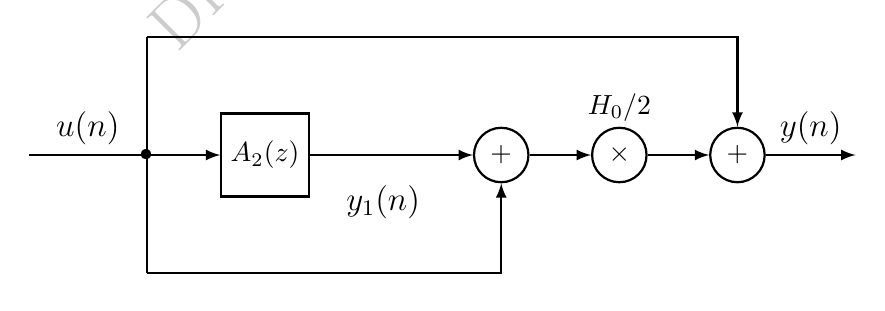
\begin{tikzpicture}[auto, thick, node distance=0.6cm, >=latex, scale = 0.75]
	\draw
	node at (2,0)[delay] (d1) {$A_2(z)$}
	node at (6,0)[sum] (s1) {$+$}
	node at (8,0)[prod](p1){$\times$} node[above of = p1]{$H_0/2$}
	node at (10,0)[sum](s2){$+$}
	node at (4,0)(n1){}
	node[below of =n1]{\large$y_1(n)$}
	;
	
	\draw[-](-2,0) -- node {\large$u(n)$}(0,0);
	\draw[->](0,0) -- node {} (d1);
	\draw[->](d1) -- node {} (s1);
	\draw[-](0,0) -- node {} (0,-2);
	\draw[->](0,-2) -| node {} (s1);
	\draw[->](s1) -- node {} (p1);
	\draw[->](p1) -- node {} (s2);
	\draw[->](s2) -- node {\large$y(n)$} (12,0);
	\draw[-](0,0) -- node {} (0,2);
	\draw[->](0,2) -| node {} (s2);
	
	\draw
	node at (0,0) {\textbullet};
	\end{tikzpicture}
\end{center}
which leads to the difference equations
\[
x(n) = u(n) - d(1 - c_{B/C})x(n - 1) + c_{B/C}x(n - 2)
\]
\[
y_1(n) = -c_{B/C}x(n) + d(1 - c_{B/C})x(n - 1) + x(n - 2)
\]
\[
y(n) = \frac{H_0}{2}[u(n) - y_1(n)] + u(n),
\]
and corresponding state and output equations are
\[
\begin{bmatrix}x(n)\\x(n-1)\end{bmatrix} = \begin{bmatrix}
-d(1-c_{B/C})&c_{B/C}\\
1&0
\end{bmatrix}
\begin{bmatrix}x(n-1)\\x(n-2)\end{bmatrix} + \begin{bmatrix}1\\0\end{bmatrix}
u(n)
\]
\[
y(n) = \begin{bmatrix}\frac{H_0}{2}(c_{B/C}^2-1)d&\frac{H_0}{2}(c_{B/C}^2-1)\end{bmatrix}
\begin{bmatrix}x(n-1)\\x(n-2)\end{bmatrix} + [\frac{H_0}{2}(1+c_{B/C})+1]u(n).
\]
The center frenquency parameter $d$ and the coefficient $H_0$ are given by
\[
d = -\cos(2\pi f_c/f_S)
\]
\[
V_0 = H(e^{j2\pi f_c/f_S}) = 10^{G/20}
\]
\[
H_0 = V_0 - 1.
\]
The bandwidth $f_b$ is adjusted through the parameters $c_B$ and $c_C$ for boost and cut given by
\[
c_B = \frac{\tan(\pi f_b/f_S) - 1}{\tan(\pi f_b/f_S) + 1}
\]
\[
c_C = \frac{\tan(\pi f_b/f_S) - V_0}{\tan(\pi f_b/f_S) + V_0}.
\]
A possible peak filter implementation using this approach is given in the following {\bfseries Matlab} code.
\begin{lstlisting}
function y = peakfiltunit(audio, para)
% Applies a peak filter to the input signal.
% para(1) is the normalized center frequency in (0,1), i.e. 2*fc/fs.
% para(2) is the normalized bandwidth in (0,1), i.e. 2*fb/fs.
% prar(3) is the gain in dB.
V0 = 10^(para(3)/20); H0 = V0 - 1;
if para(3) >= 0
	c = (tan(pi* para(2)/2)-1) / (tan(pi* para(2)/2)+1);     % boost
else
	c = (tan(pi* para(2)/2)-V0) / (tan(pi* para(2)/2)+V0);   % cut
end;
d = -cos(pi*para(1));
x = [0; 0];
x_1 = 0;
A = [-d*(1-c), c; 1, 0];
B = [1; 0];
C = [H0/2*(c^2-1)*d, H0/2*(c^2-1)];
D = [H0/2*(1+c) + 1];
for n=1:length(audio)
	x_1 = A * x + B * audio(n);
	y(n) = C * x + D * audio(n);
	x = x_1;
end
\end{lstlisting}
\end{document}
